\documentclass[12pt,a4paper]{article}
\usepackage[utf8]{inputenc}
\usepackage{geometry}
\usepackage{titlesec}
\usepackage{fancyhdr}
\usepackage{setspace}
\usepackage{graphicx} % For including images
\usepackage{float} % For figure placement
\usepackage{hyperref}
\usepackage{subcaption}
\usepackage{placeins} % Add in the preamble for \FloatBarrier



% Page Setup
\geometry{margin=1in}
\setstretch{1.25}

% Header and Footer
\pagestyle{fancy}
\fancyhf{}
\fancyhead[L]{Hotel Management System Project Report}
\fancyfoot[C]{\thepage}

% Title Formatting
\titleformat{\section}{\large\bfseries}{\thesection}{1em}{}
\titleformat{\subsection}{\normalsize\bfseries}{\thesubsection}{1em}{}

% Title Information
\title{
    \vspace{1in}
    \textbf{\Huge Hotel Management System Project Report}\\[1cm]
    \normalsize A project submitted by:\\[0.5cm]
    \large Umais Ahmed (24K-2043), Zumair Shamsi (24K-2040), Ali Safir (24K-2039),\\
    Aayan Sultan (24K-2015), Humayun Shahid (24K-2011)\\[1in]
    \textbf{\today}\\[1in]
}
\date{}
\author{}

\begin{document}

\maketitle
\newpage

\tableofcontents
\newpage

\section{Introduction}
This report outlines the development and implementation of the \textit{Hotel Management System}, a project designed to automate hotel operations such as guest booking, room management, and administrative tasks. The system was built using the \textbf{C programming language}, incorporating file handling to ensure data persistence and effective management.

\section{Background}
\subsection{Research}
During the project, we explored advanced concepts of the C programming language, particularly format specifiers. Examples include:
\begin{itemize}
    \item \verb|%14s|: Allocates exactly 14 spaces for the string, useful for aligning text in tables or reports.
    \item \verb|%-10d|: Left-aligns an integer within 10 spaces for better readability.
    \item \verb|%.2f|: Formats a float to show exactly 2 decimal places, ensuring precision in numerical outputs.
\end{itemize}
Learning these advanced specifiers improved the clarity and professionalism of our system's output.

\subsection{BROgramming Initiative}
Our senior peers in the \textit{BROgramming Initiative} were instrumental in our success. They provided guidance on:
\begin{itemize}
    \item Writing efficient, clean, and modular code.
    \item Understanding and implementing complex logic.
    \item Debugging and optimizing our program for better performance.
\end{itemize}
Their mentorship significantly enhanced our coding practices and problem-solving skills.
\newpage
\section{Specifications}
\subsection{Tools Used}
\begin{itemize}
    \item \textbf{Programming Language}: C
    \item \textbf{Compiler}: MinGW
    \item \textbf{IDE}: Visual Studio Code / Dev C++
    \item \textbf{Libraries}: Standard C library for input/output and file handling.
    \item \textbf{Platform}: Windows
\end{itemize}

\section{Problem Analysis}
The hotel industry faces challenges with outdated, expensive, and complex systems. Smaller hotels struggle with cost and usability barriers. We decided to create a text-based system in C to address these gaps.

\section{Solution Design}
\subsection{Function Call Hierarchy}
The figure below outlines the hierarchy of function calls within the system:
\begin{figure}[H]
    \centering
    \includegraphics[width=0.8\textwidth]{graph.png} % Updated image path
    \caption{Function Call Hierarchy (Tree Layout)}
    \label{fig:hierarchy}
\end{figure}

\subsection{Functionality and Features}
\begin{itemize}
    \item \textbf{Guest Functions}: Login/Sign-up, room browsing, room booking, service requests, and feedback submission.
    \item \textbf{Admin Functions}: Room management (add, modify, delete), reservation management, and report generation.
    \item \textbf{File Handling}: Persistent data storage using files for guest, room, and reservation information.
\end{itemize}

\section{Implementation \& Testing}
\subsection{Implementation Overview}
The system uses modular functions for tasks like room booking, reservation management, and report generation. File handling ensures data persistence between sessions.

\subsection{Testing}
We tested:
\begin{itemize}
    \item Room availability checks and booking logic.
    \item File operations for data integrity.
    \item User input validation to prevent errors.
\end{itemize}

\section{Project Breakdown Structure}
\subsection{Workload Distribution}
\begin{itemize}
    \item \textbf{Umais Ahmed, Ali Safir}: Admin functionalities. Implemented adding, modifying, and deleting rooms, managing reservations, and generating reports. Also managed file handling
      \item \textbf{Zumair Shamsi, Humayun Shahid}: Worked on guest functionalities, such as user login, room booking, and feedback submission. Also ensured that the guest interface was user-friendly and functional.
    \item \textbf{Aayan Sultan}: Team Lead, ensured smooth coordination among team members, handled testing and debugging. Maintained Git repository, task distribution, and creating the report.

\end{itemize}

\clearpage

\subsection{Timeline}
\begin{itemize}
    \item \textbf{Day 1-2}: Requirements gathering and initial system design.
    \item \textbf{Day 3-8}: Development of guest and admin functionalities.
    \item \textbf{Day 9-10}: Testing, debugging, and file handling validation.
    \item \textbf{Day 11-12}: Final revisions and documentation.
\end{itemize}

\section{Results}
\subsection{System Output}
The system provides features like:
\begin{itemize}
    \item Real-time room availability checks.
    \item Accurate reservation tracking.
    \item Simple file-based data management.
\end{itemize}

\section{Conclusion}
The \textit{Hotel Management System} project provided practical exposure to C programming concepts like modular design, file handling, and debugging. The system meets its objectives, with room for improvement in GUI and online booking.

\subsection{Discussion}
Future enhancements include:
\begin{itemize}
    \item Adding a graphical user interface (GUI).
    \item Integrating real-time booking with online functionality.
    \item Expanding reporting capabilities for better analytics.
\end{itemize}

\clearpage
\vspace{0.5em}

\subsection{Images}

\subsubsection{User Views}
% Individual images
\begin{figure}[!htbp]
    \centering
    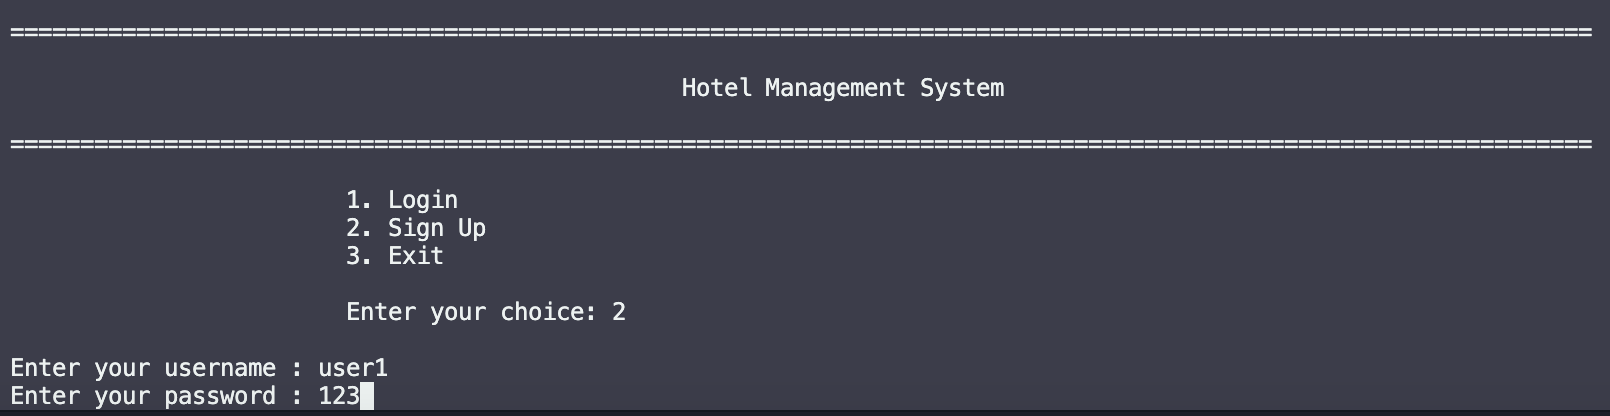
\includegraphics[width=\linewidth]{user-login.png} % User login
    \caption{User Login Page.}
\end{figure}

\begin{figure}[!htbp]
    \centering
    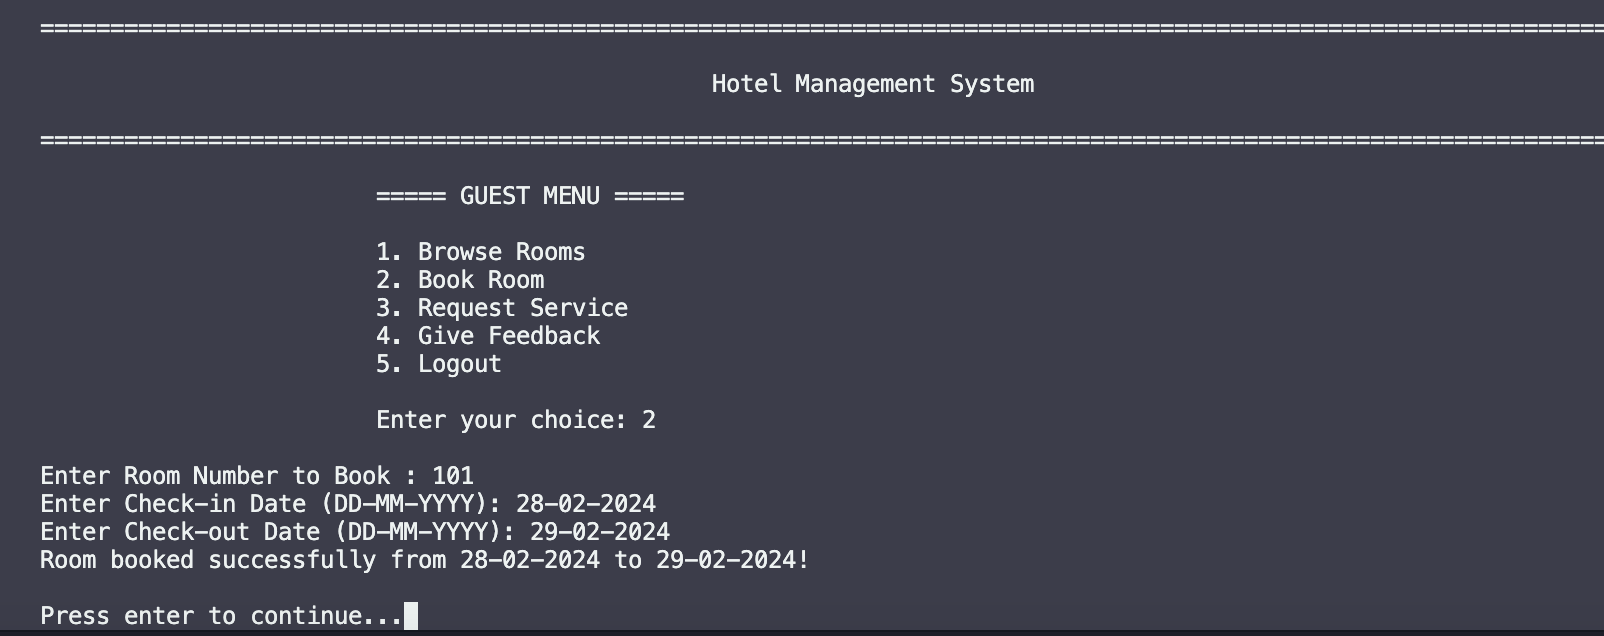
\includegraphics[width=\linewidth]{booking.png} % User booking
    \caption{User Booking Interface.}
\end{figure}

\begin{figure}[!htbp]
    \centering
    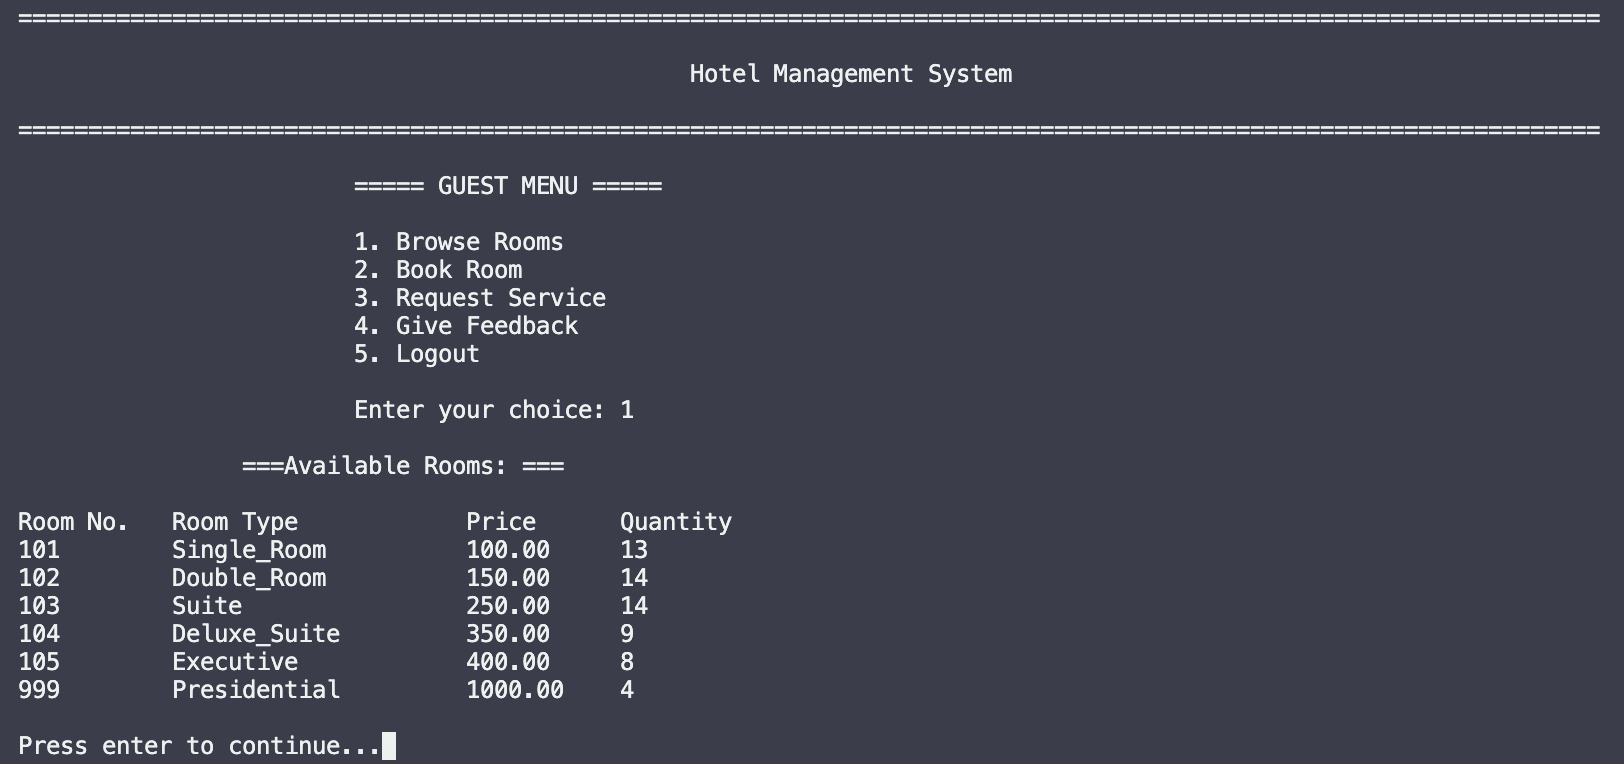
\includegraphics[width=\linewidth]{browse.png} % Browsing rooms
    \caption{Browsing Available Rooms.}
\end{figure}

\begin{figure}[!htbp]
    \centering
    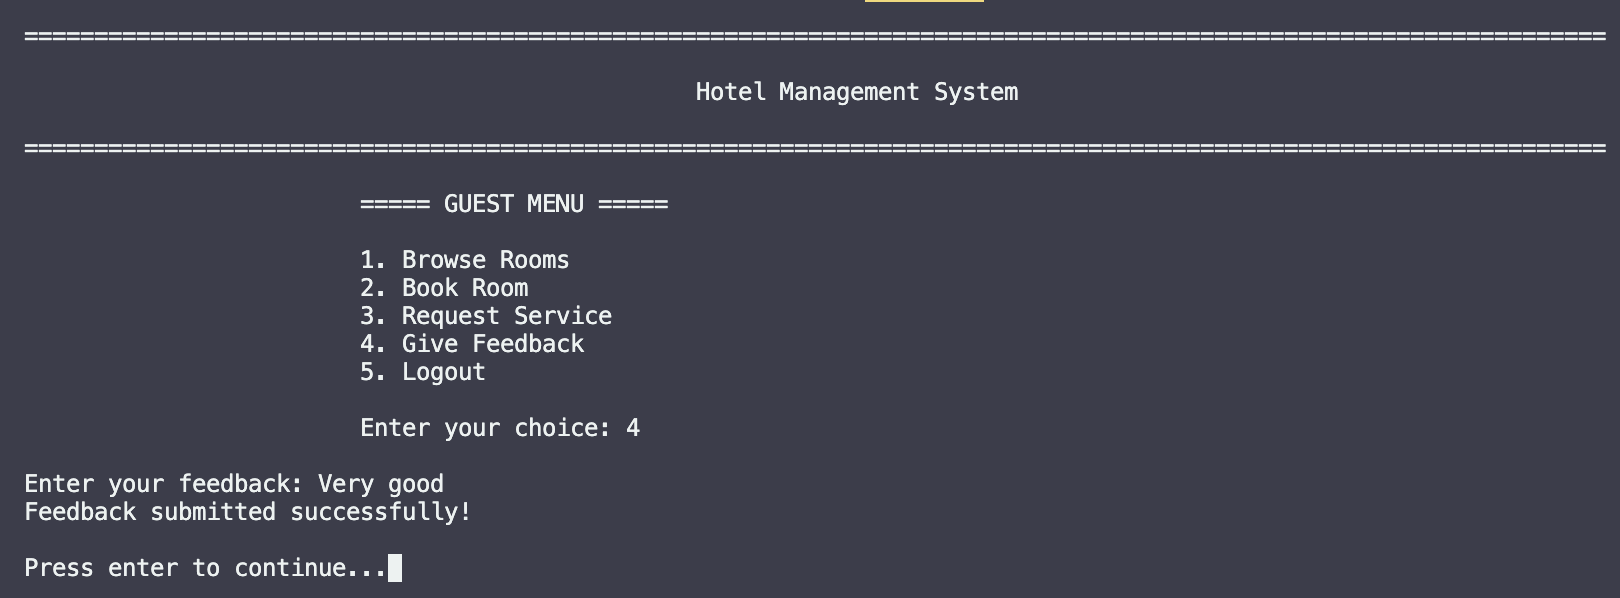
\includegraphics[width=\linewidth]{feedback.png} % Feedback interface
    \caption{Room Feedback Interface.}
\end{figure}
\clearpage
\subsubsection{Admin Panel}
% Individual images
\begin{figure}[!htbp]
    \centering
    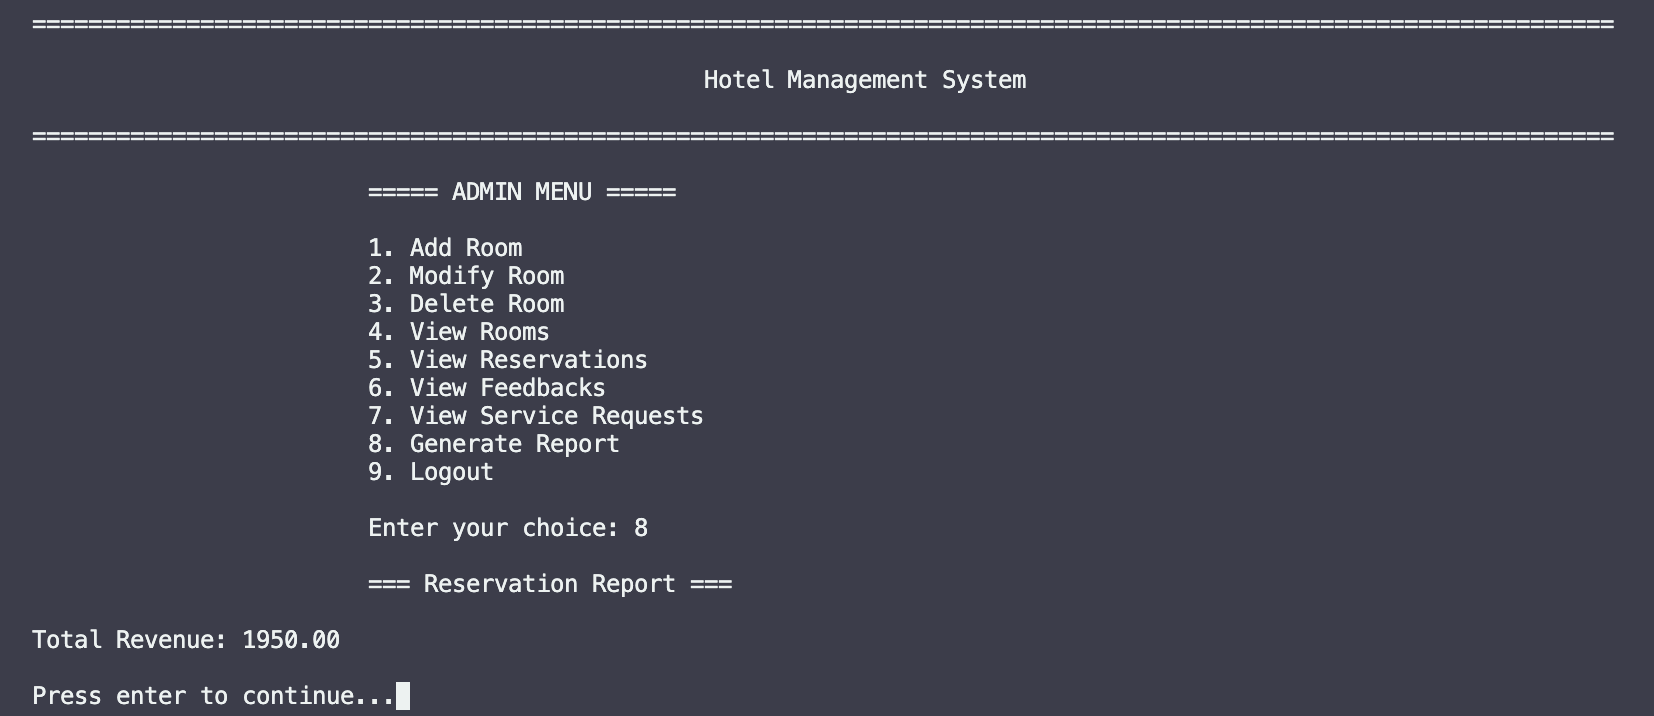
\includegraphics[width=\linewidth]{admin.png} % Admin panel
    \caption{Admin Panel Overview.}
\end{figure}

\begin{figure}[!htbp]
    \centering
    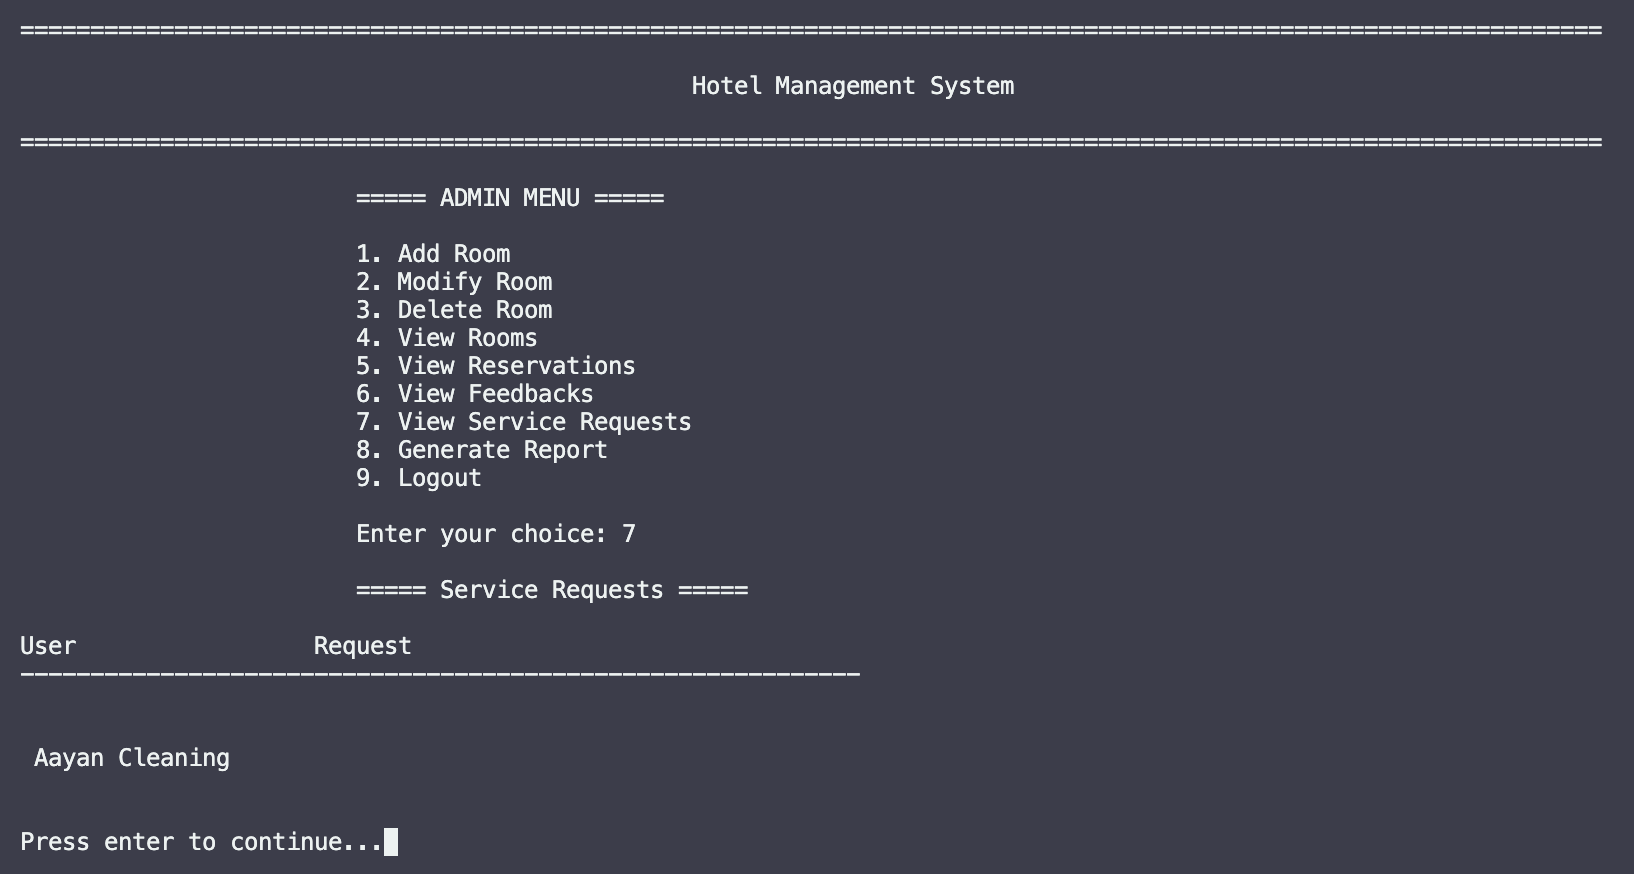
\includegraphics[width=\linewidth]{admin-service.png} % Feedback system
    \caption{Feedback View on Admin Side.}
\end{figure}

\begin{figure}[!htbp]
    \centering
    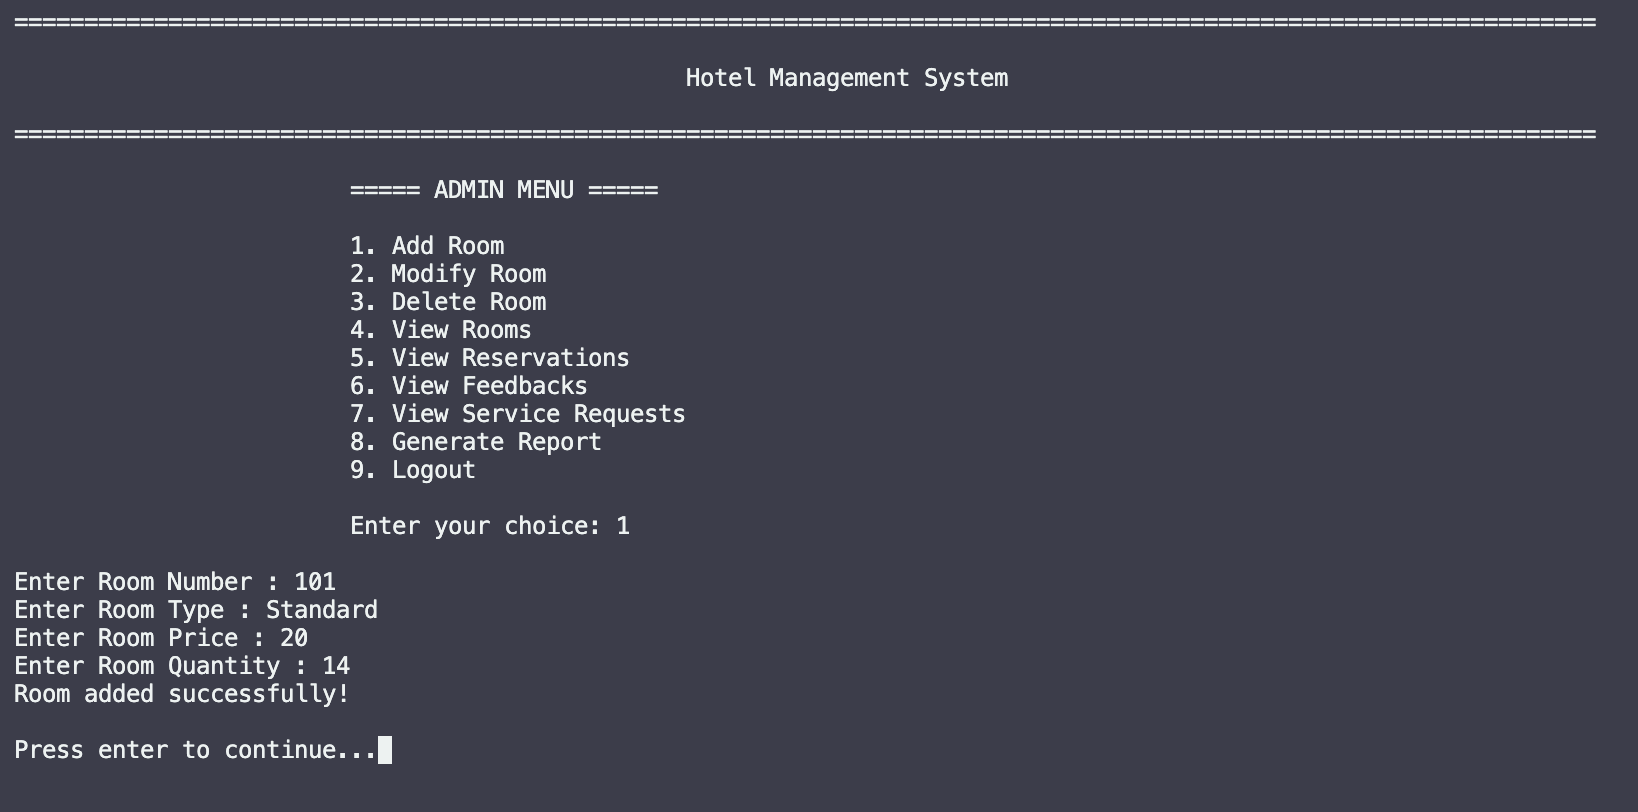
\includegraphics[width=\linewidth]{room_add.png} % Admin room add
    \caption{Admin Room Add Interface.}
\end{figure}

\begin{figure}[!htbp]
    \centering
    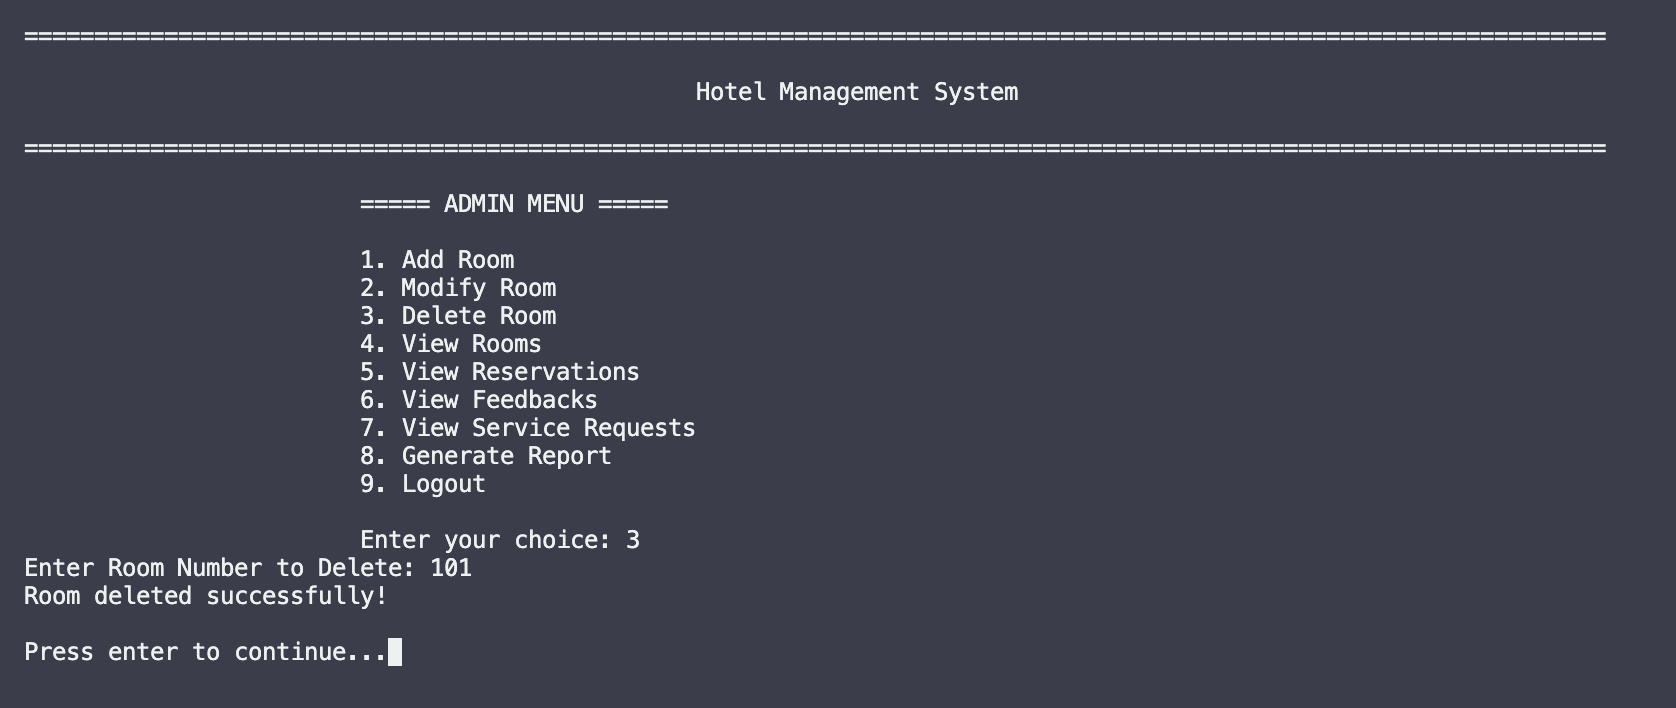
\includegraphics[width=\linewidth]{room_delete.png} % Admin room delete
    \caption{Admin Room Delete Interface.}
\end{figure}




\end{document}
